\Needspace{14\baselineskip}
\section{A complete two-channel decision for the source family}
\label{sec:twochannel}


The single square-root cutoff in Proposition~\ref{prop:30241} can be
completed by a second search in the auxiliary parameter $k$.
The second congruence description below is the $a=1$ case of the
first Type~I family in Elsholtz and Tao
\cite[Proposition~1.9]{ET}.

\begin{theorem}[Two-channel completeness]\label{thm:twochannel}
Let $p\equiv1\pmod4$ be prime, and put
\[
 K=\left\lfloor\sqrt{\frac{p+1}{4}}\right\rfloor .
\]
There is a source witness \eqref{eq:source} with $1\le i<p$ if and
only if at least one of the following two finite searches succeeds.
\begin{enumerate}
\item For some $1\le i\le K+1$, a divisor $d\mid p+i$ satisfies
      $d\equiv3\pmod4$ and $4i\mid p+d$.
\item For some $1\le k\le K$, a divisor $d\mid4k+1$ satisfies
      $d\equiv3\pmod4$ and $4k\mid p+d$.
\end{enumerate}
More precisely, every witness of the unrestricted source search is
represented in one of these two branches, with the same $d$ and
$k=(p+d)/(4i)$. A witness from the second branch gives the source
index $i=(p+d)/(4k)$.
\end{theorem}
\begin{proof}
Take any source witness and set $k=(p+d)/(4i)\in\mathbb N$.
Any common divisor of $d$ and $i$ divides $p$, because
$d\mid p+i$. Since $i<p$ and $p$ is prime, this proves
$\gcd(d,i)=1$. The two relations
$d\mid p+i$ and $p+d=4ik$ give
\[
 d\mid i(4k+1).
\]
Coprimality implies $d\mid4k+1$, hence $d\le4k+1$. Therefore
\begin{equation}\label{eq:source-hyperbola}
 (i-1)k=\frac{p+d-4k}{4}\le\frac{p+1}{4}.
\end{equation}
If $i\ge K+2$ and $k\ge K+1$, the left side is at least
$(K+1)^2>(p+1)/4$, a contradiction. Thus $i\le K+1$ or
$k\le K$. The boundary case $i=1$ is included in the first
branch directly, and \eqref{eq:source-hyperbola} still holds.

A witness in the first branch already meets the source conditions,
and $K+1<p$ for every prime $p\equiv1\pmod4$.
For a witness in the second branch, $i=(p+d)/(4k)$ is a positive
integer. Since $d\le4k+1$ and $k\ge1$,
\[
 i\le\frac{p}{4k}+1+\frac1{4k}
   \le\frac{p+5}{4}<p.
\]
Also $p+i=i(4k+1)-d$ is divisible by $d$, while
$4i\mid p+d$ follows from $p+d=4ik$. Along with
$d\equiv3\pmod4$, these are exactly \eqref{eq:source}.
\end{proof}

For the prime $p=30241$, one has $K=86$. Its first source
$i=161$ is visible in the second branch through $k=47$ and $d=27$,
since
\[
 4\cdot47+1=189=7\cdot27,\qquad
 30241+27=4\cdot47\cdot161.
\]
There is also a second-branch witness $k=19$, $d=7$,
corresponding to the source $i=398$.

\begin{figure}[htbp]
\centering
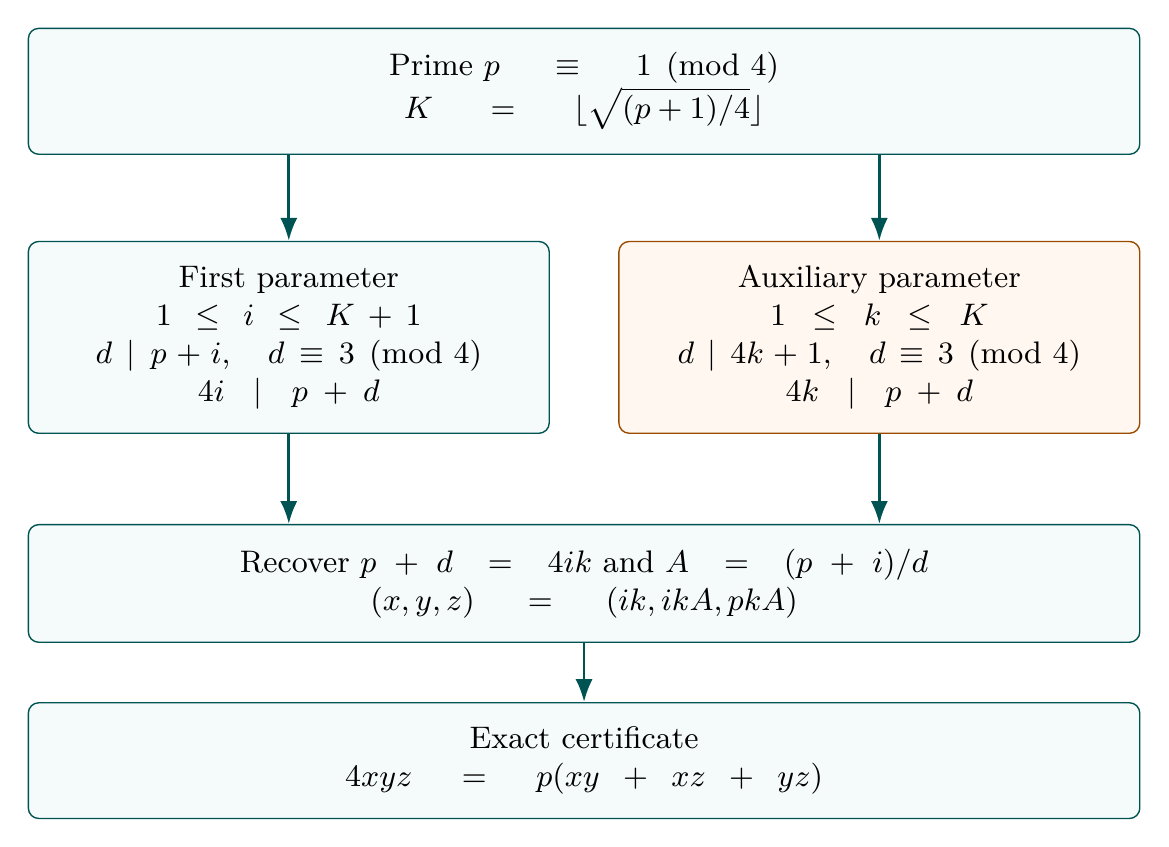
\includegraphics[width=.94\linewidth]{source-search/figures/two-channel-flow.png}
\caption{The two finite searches in Theorem~\ref{thm:twochannel}.
Every successful branch gives an exact unit-fraction certificate.}
\label{fig:twochannel}
\end{figure}

\begin{figure}[htbp]
\centering
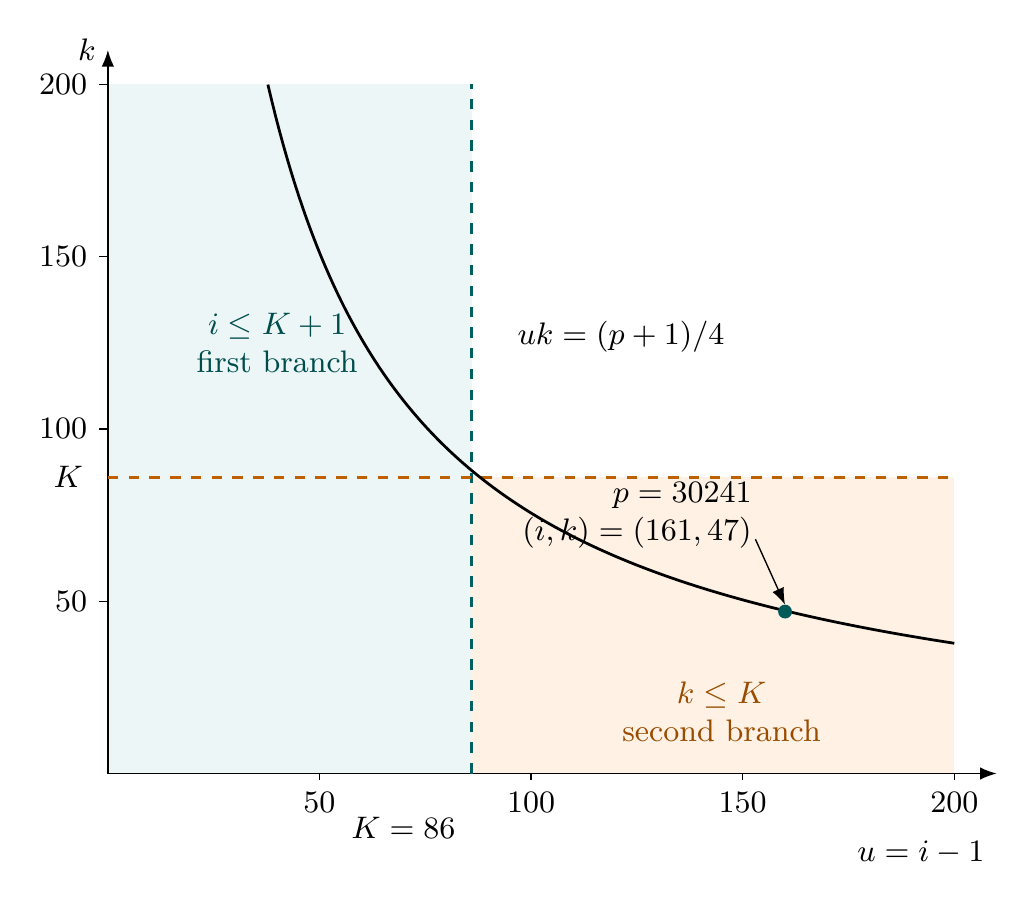
\includegraphics[width=.72\linewidth]{source-search/figures/source-hyperbola.png}
\caption{The necessary parameter bound for $p=30241$.
The shaded strips represent the two finite budgets.
The displayed witness has $i=161$ and $k=47$.
The curve is a necessary envelope, with the divisor
congruences also required for an integer point to be a witness.}
\label{fig:hyperbola}
\end{figure}

The theorem gives a complete decision procedure for the specified
$a=1$ source family using $K+1$ source indices and $K$ auxiliary
indices, with divisor enumeration at each index. The assertion that
one of these finite branches succeeds for every remaining prime is
a further nonemptiness problem. The equivalence itself imposes no
claim about its answer.
